% TEX root = main.tex
\section{Introduction}

The \underline{W}eb\underline{A}ssembly \underline{S}ymbolic \underline{P}rocessor, WASP, is a novel concolic execution engine for testing Wasm (version 1.0) modules.
WASP follows the so-called \emph{concolic discipline}~\cite{Godefroid:2005,Sen:2005}, combining concrete execution with symbolic execution and exploring one execution path at a time.
However, unlike most concolic execution engines~\cite{multi-se,you:esop:2021,Sen:2005,sen:cav:2006}, which are implemented via program instrumentation, we implement WASP by instrumenting the Wasm reference interpreter developed by Haas et al.~\cite{Haas:2017}. To this end, we lift the authors' reference interpreter from concrete values to pairs of concrete and symbolic values. 
By moving the instrumentation to the interpreter level, we open up the possibility for a range of optimisations in the context of concolic execution, such as application of algebraric simplification to byte-level symbolic expressions and shortcut restarts for failed assumption statements~\cite{marques:2022}.

While our first goal is for WASP to be able to analyse stand-alone Wasm modules, we also aim for it to be used as a common platform for building symbolic analyses for high-level programming languages that compile to Wasm. In order to demonstrate the viability of this approach, we use it to build WASP-C, a new symbolic execution framework for testing C programs. WASP-C shows that, with a relatively small effort ($\approx800$ LoC), we were able to build a new concolic engine for C that is able to analyse industry-grade code and obtain results comparable to well-established symbolic execution and testing tools for C, such as KLEE~\cite{Cadar:2008} and VeriFuzz~\cite{BasakC:2019}.

\section{Our Approach}

In this section we explore the theoretical underpinnings of the technique used by WASP and compre it with existing symbolic analysis tools for WebAssembly.

\paragraph{Symbolic Execution.}
Symbolic execution has been extensively used to find crucial errors and vulnerabilities in a broad spectrum of programming languages, such as C~\cite{Godefroid:2005}, C++~\cite{Cadar:2008}, Java~\cite{Sen:2005}, and~Python~\cite{Chen:2014}. Regarding the Web, there are several state-of-the-art tools for symbolically executing JavaScript code~\cite{cosette,javert2.0,sym-exec-framework-for-javascript,symjs,multi-se}, demonstrating the need for such tools for the validation and testing of modern Web applications.

Symbolic execution tools can be divided into two main classes: \emph{static} and \emph{dynamic/concolic}~\cite{survey}. Static symbolic execution engines, such as~\cite{effigy,Pasareanu:2010,generalized-sym-exec,rosette,cosette,javert2.0}, explore the entire symbolic execution tree up to a pre-established depth, while concolic execution engines, such as~\cite{Cadar:2008,Godefroid:2005,Sen:2005,mayhem,sym-exec-framework-for-javascript,symjs,multi-se}, usually work by pairing up a concrete execution with a symbolic execution and exploring one execution path at a time. An advantage of concolic execution over static symbolic execution is that concolic execution requires less frequent interactions with the solver and a simpler memory model. There is a vast body of research on both static and concolic symbolic execution tools for a wide variety of programming languages, see~\cite{survey,survey1,sym-exec-3-decades-later} for comprehensive surveys on the topic. In the following, we give a detailed account of the only two existing symbolic execution tools for Wasm other than WASP. 

WANA~\cite{Wang:2020} is a cross-platform smart contract vulnerability detection tool employed to find vulnerabilities in EOSIO~\cite{Larimer:2018} and Ethereum smart contracts~\cite{Kashyap:2021}. WANA is based on static symbolic execution and operates over Wasm bytecode. To detect vulnerabilities in smart contracts, WANA comes with three heuristics for EOSIO smart contracts and four for Ethereum smart contracts.
 Unlike WASP, WANA lacks a stand-alone symbolic execution engine for Wasm. Hence, it is not possible to run WANA on arbitrary Wasm code without refactoring its internal architecture. For this reason, we were unable to evaluate WANA and compare its performance with those of WASP and Manticore.  

Manticore~\cite{Mossberg:2019} is a symbolic execution framework for binaries and smart contracts. Manticore is highly flexible, supporting a wide range of binaries and computing environments, including Wasm bytecode. % e.g., it supports ELF binaries for x86/64 and ARM, Ethereum smart contracts for the Ethereum platform, and, as of recently, Wasm bytecode. Manticore 
%It implements various \ti{native execution models} for the execution environments that it supports; these models then interact with a generic platform-agnostic symbolic execution engine. 
When it comes to Wasm, Manticore does not expose dedicated primitives for constructing and reasoning over symbolic values at the source language level. Symbolic inputs and constraints are created as part of a complex Python script that must be written for each test~\cite{Hennenfent:2020}, which initialises the symbolic state and calls the appropriate Wasm module. This process does not scale for a broad evaluation, as one would have to manually write a python script for each symbolic test. Nonetheless, we compare the performance of WASP with that of Manticore~\cite{Mossberg:2019} in the analysis of a stand-alone Wasm implementation of a B-tree data structure, demonstrating that WASP is consistently faster.

\section{Tool Architecture}

\begin{figure}[t!]
  \centering
  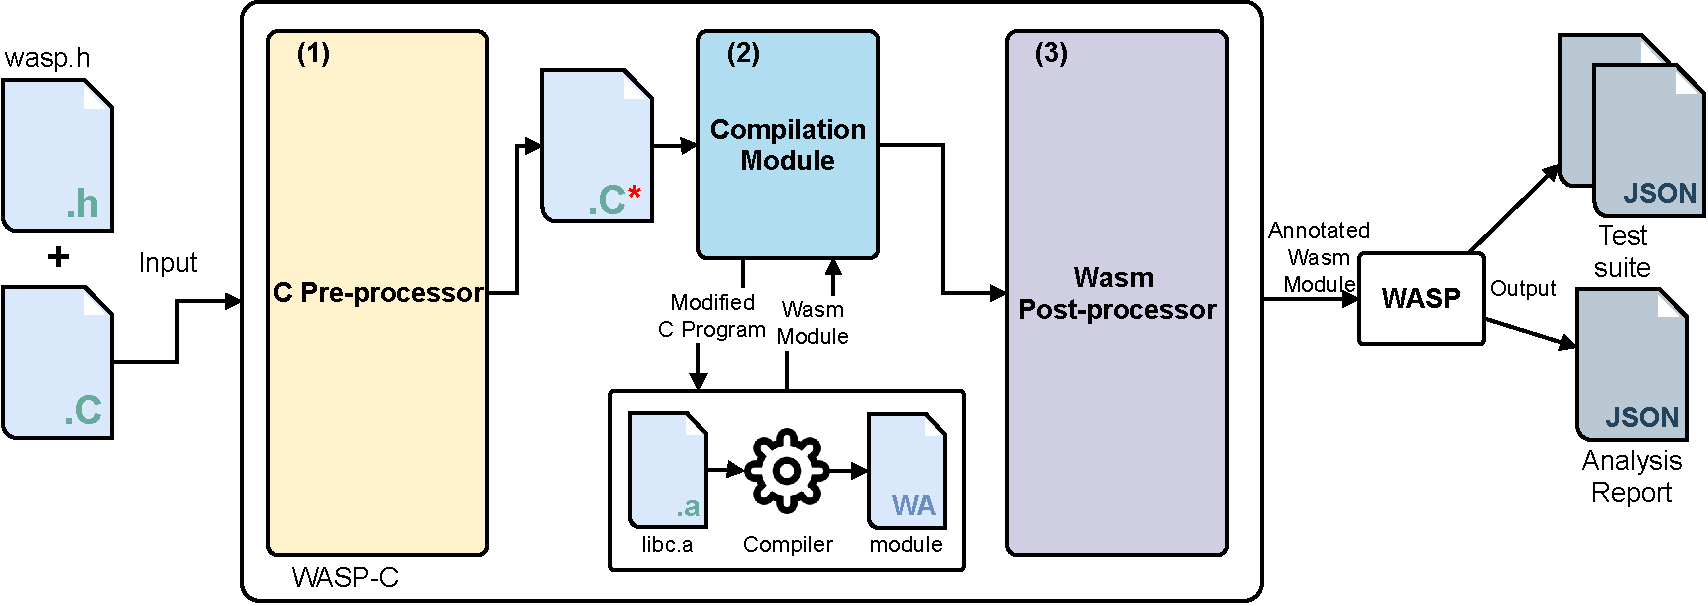
\includegraphics[width=0.9\linewidth]{graphics/wasp-c}
  \caption{High-level architecture of WASP-C.}%
  \label{fig:arch}
\end{figure}

WASP-C takes as input C programs annotated with assumptions and assertions and outputs a \textit{test suite}. A test suite is a list of test cases, each corresponding to a JSON file, mapping the symbolic variables in the test to their corresponding concrete values. Each test case captures a different execution path of the program to be analysed. Since WASP does not directly operate over the C source code, WASP-C is comprised of three modules whose end goal is to generate a Wasm program for WASP to analyse.

WASP-C is implemented in python and is composed of three essential modules: a \textit{C Pre-processor}, a \textit{Compilation Module}, and a \textit{Wasm Post-processor}, which interact with each other according to the high-level architecture described in Figure~\ref{fig:arch}.
Using WASP as a submodule, WASP-C concolically executes C programs as follows.
First, the \textit{C Pre-processor} parses the given program using a standard C parser called \textit{pycparser},\footnote{\url{https://github.com/eliben/pycparser}} generating an abstract syntax tree (AST) that is then sent to a specialised C visitor (step 1). Our specialised C visitor traverses the AST, replacing binary operators such as logical ANDs and ORs with specific function calls to avoid spurious branching. Then the AST is exported back to a C program, which is subsequently compiled into Wasm by the \textit{Compilation Module} (step 2). Lastly, the \textit{Wasm Post-processor} processes the obtained Wasm module so as to inject the appropriate WASP symbolic primitives~(step~3).

\section{Strengths and Weaknesses}

The main strength of WASP is that it can quickly generate inputs that trigger assertion violations in the program. For WASP-C's evaluation we tested WASP-C against the benchmark suite of Test-Comp 2021. For the \texttt{cover-error} meta-category WASP-C was able to score 360 points which would have yield a third-place in Test-Comp 2021.

WASP only implements standard branch search policies, such as DFS, BFS, and random selection; therefore, WASP has difficulties in generating high-coverage test suites.

\section{Tool Configuration and Setup}

WASP and WASP-C are publicly available at the URL \url{https://github.com/wasp-platform/wasp}. Its Test-Comp 2023 variant is available at the URL \url{blah bleh}. The benchmark description file is \texttt{wasp-c.xml}. To install and run the tool, follow the instructions provided in \texttt{README.md}. A sample run command is as follows:

\begin{minted}[fontsize=\footnotesize,breaklines]{sh}
./bin/wasp-c --smt-assume --policy breadth --test-comp -p cover-error.prp examples/CostasArray-10.c
\end{minted}

\section{Software Project and Contributors}

WASP and WASP-C is developed by the authors and their students. We would also like thank Carolina Costa with whom we designed a preliminary version of~WASP\@.
